\chapter{Day 2 Motions}
\label{ch-day2}




% ******************************************************************
% ******************************************************************
% ******************************************************************
\clearpage
\newpage
\section{Deconvolution 1D Motions}
\label{Deconvolution_1D_Motions}


\subsection{Free field 1D model, deconvolution 1D motion, model with DRM}
\label{Free_fields_1D_model_with_DRM1}


The Real-ESSI input files for this example are available 
\href{http://sokocalo.engr.ucdavis.edu/~jeremic/lecture_notes_online_material/_Chapter_Short_Course_Examples/Day2/Deconvolution_1D_Motions/Free_fields_1D_model_with_DRM}{HERE}. 
The compressed package of Real-ESSI input files for this example is available 
\href{http://sokocalo.engr.ucdavis.edu/~jeremic/lecture_notes_online_material/_Chapter_Short_Course_Examples/Day2/Deconvolution_1D_Motions/Free_fields_1D_model_with_DRM/_all_files_packaged_for_Free_fields_1D_model_with_DRM.tar.gz}{HERE}. 

The Modeling parameters are listed.
\begin{itemize}
  \item Elastic Material Properties 
  \begin{itemize}
    \item Mass density, $\rho$, \enspace \enspace 2000 $kg/m^3$
    \item Shear Wave Velocity, $V_s$, \enspace \enspace 500 $m/s$
    \item Young's modulus, $E$, \enspace \enspace 1.1 GPa
    \item Poisson's ratio, $\nu$, \enspace \enspace 0.1
  \end{itemize}
\end{itemize}


\begin{figure}[H]
  \centering
  \includegraphics[width = 0.8cm]{./Figure-files/Day2/Deconvolution_1D_Motions/Free_fields_1D_model_with_DRM/overview.png}
  \caption{Simulation Model}
  \label{fig_decon_1D_motion_1D_model1}
\end{figure}

The illustration results of the simulation is shown in Fig.~\ref{fig_decon_1D_motion_1D_model}.
As shown in the results, outside the DRM layer, there is no outgoing waves. 

\begin{figure}[H]
  \centering
  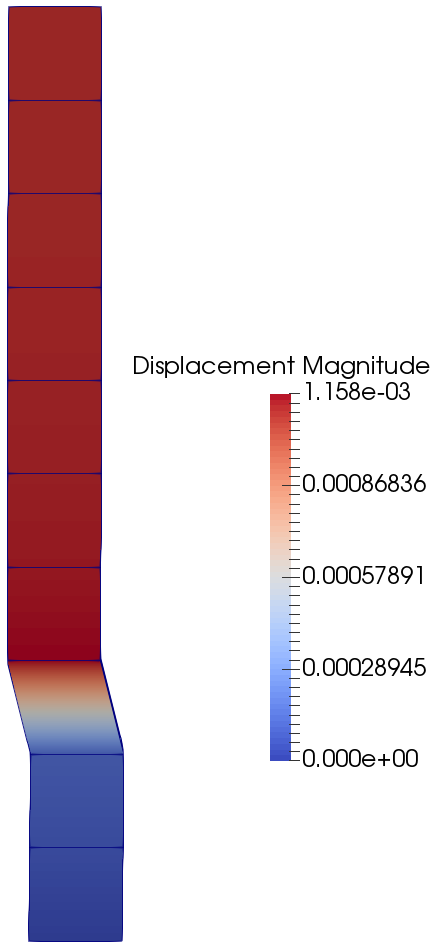
\includegraphics[width = 5cm]{./Figure-files/Day2/Deconvolution_1D_Motions/Free_fields_1D_model_with_DRM/DRM1D_results.png}
  \caption{Simulation Model}
  \label{fig_decon_1D_motion_1D_model_results}
\end{figure}


% ******************************************************************
% ******************************************************************
% ******************************************************************
\clearpage
\newpage
\subsection{Free field 3D model, deconvolution 1D motion, model with DRM}
\label{Free_fields_3D_model_with_DRM1}


The Real-ESSI input files for this example are available 
\href{http://sokocalo.engr.ucdavis.edu/~jeremic/lecture_notes_online_material/_Chapter_Short_Course_Examples/Day2/Deconvolution_1D_Motions/Free_fields_3D_model_with_DRM}{HERE}. 
The compressed package of Real-ESSI input files for this example is available 
\href{http://sokocalo.engr.ucdavis.edu/~jeremic/lecture_notes_online_material/_Chapter_Short_Course_Examples/Day2/Deconvolution_1D_Motions/Free_fields_3D_model_with_DRM/_all_files_packaged_for_Free_fields_3D_model_with_DRM.tar.gz}{HERE}. 

The Modeling parameters are listed.
\begin{itemize}
  \item Elastic Material Properties 
  \begin{itemize}
    \item Mass density, $\rho$, \enspace \enspace 2000 $kg/m^3$
    \item Shear Wave Velocity, $V_s$, \enspace \enspace 500 $m/s$
    \item Young's modulus, $E$, \enspace \enspace 1.1 GPa
    \item Poisson's ratio, $\nu$, \enspace \enspace 0.1
  \end{itemize}
\end{itemize}


\begin{figure}[H]
  \centering
  \includegraphics[width = 8cm]{./Figure-files/Day2/Deconvolution_1D_Motions/Free_fields_3D_model_with_DRM/overview.png}
  \caption{Simulation Model}
  \label{fig_decon_1D_motion_3D_model1}
\end{figure}


The illustration results of free field DRM 3D Model under 1D motion is shown 
in Fig.~\ref{fig_day2_DRM3D_results}. 

\begin{figure}[H]
  \centering
  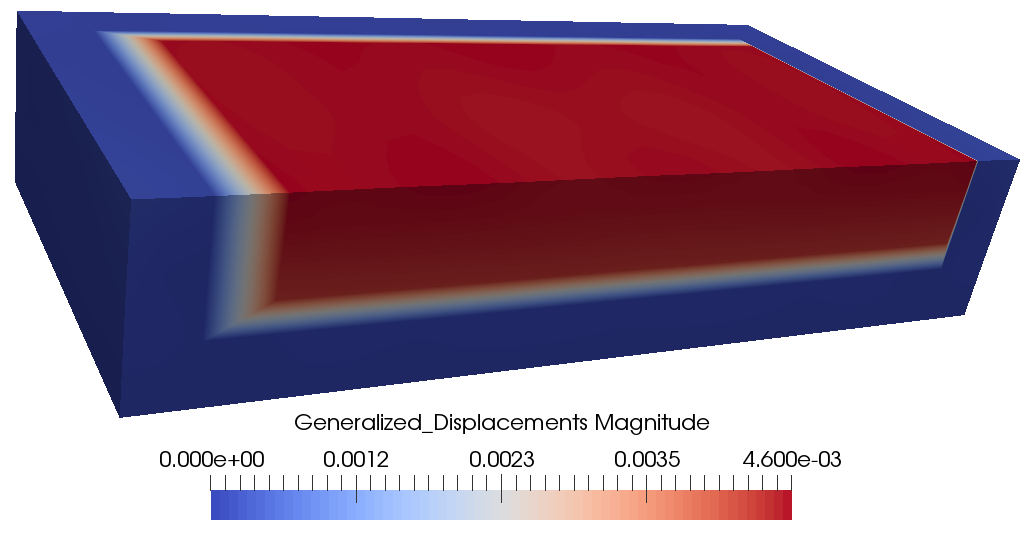
\includegraphics[width = 10cm]{./Figure-files/Day1/Preprocess_examples_with_Gmsh/example4/DRM3D_results.png}
  \caption{Simulation Model DRM 2D}
  \label{fig_day2_DRM3D_results}
\end{figure}



% % ******************************************************************
% % ******************************************************************
% % ******************************************************************
% \clearpage
% \newpage
% \subsection{ESSI 3D building model, deconvolution 1D model, solid model with DRM}
% \label{Earthquake_Soil-Structure_Interaction_3D_Model_with_DRM1}

% The Real-ESSI input files for this example are available 
% \href{http://sokocalo.engr.ucdavis.edu/~jeremic/lecture_notes_online_material/_Chapter_Short_Course_Examples/Day2/Deconvolution_1D_Motions/Earthquake_Soil-Structure_Interaction_3D_Model_with_DRM}{HERE}. 
% The compressed package of Real-ESSI input files for this example is available 
% \href{http://sokocalo.engr.ucdavis.edu/~jeremic/lecture_notes_online_material/_Chapter_Short_Course_Examples/Day2/Deconvolution_1D_Motions/Earthquake_Soil-Structure_Interaction_3D_Model_with_DRM/_all_files_packaged_for_Earthquake_Soil-Structure_Interaction_3D_Model_with_DRM.tar.gz}{HERE}. 

% The Modeling parameters are listed.
% \begin{itemize}
%   \item Elastic Soil Material Properties 
%   \begin{itemize}
%     \item Mass density, $\rho$, \enspace \enspace 2000 $kg/m^3$
%     \item Shear Wave Velocity, $V_s$, \enspace \enspace 500 $m/s$
%     \item Young's modulus, $E$, \enspace \enspace 1.1 GPa
%     \item Poisson's ratio, $\nu$, \enspace \enspace 0.1
%   \end{itemize}
%   \item Elastic Structure Material Properties 
%   \begin{itemize}
%     \item Mass density, $\rho$, \enspace \enspace 2500 $kg/m^3$
%     \item Young's modulus, $E$, \enspace \enspace 20 GPa
%     \item Poisson's ratio, $\nu$, \enspace \enspace 0.1
%   \end{itemize}
% \end{itemize}

% \begin{figure}[H]
%   \centering
%   \includegraphics[width = 8cm]{./Figure-files/Day2/Deconvolution_1D_Motions/Earthquake_Soil-Structure_Interaction_3D_Model_with_DRM/overview.png}
%   \caption{Simulation Model}
%   \label{fig_decon_1D_motion_3D_model2}
% \end{figure}


% The illustration results of DRM 3D Solid Structure Model  under 1D motion is shown 
% in Fig.~\ref{fig_decon_1D_motion_3D_model_solid_structure}. 

% \begin{figure}[H]
%   \centering
%   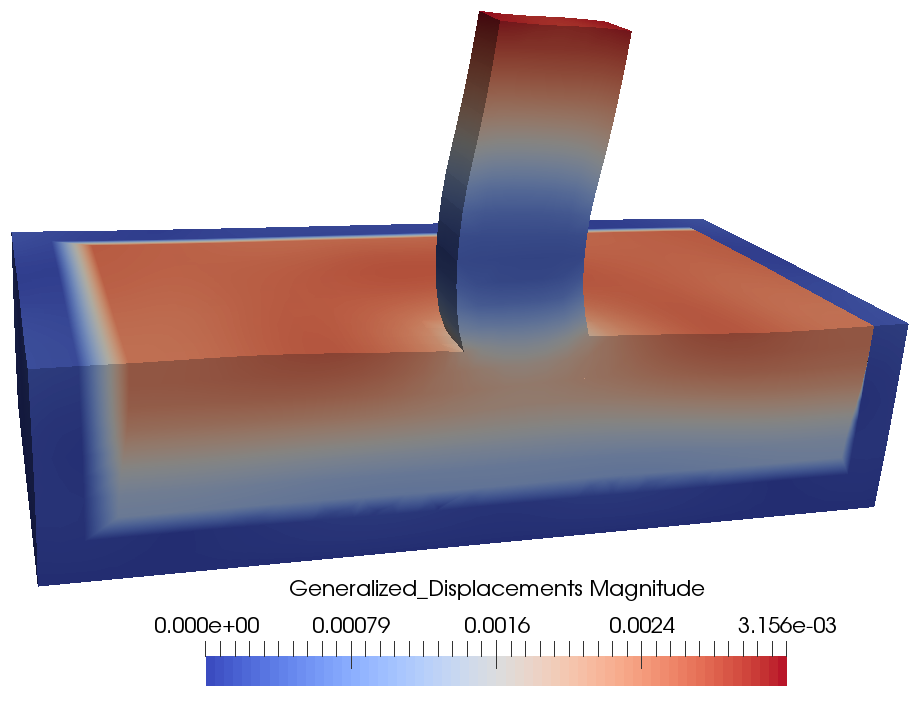
\includegraphics[width = 10cm]{./Figure-files/Day2/Deconvolution_1D_Motions/Earthquake_Soil-Structure_Interaction_3D_Model_with_DRM/DRM3D_results_1Dmotion.png}
%   \caption{Simulation Model}
%   \label{fig_decon_1D_motion_3D_model_solid_structure}
% \end{figure}






% ******************************************************************
% ******************************************************************
% ******************************************************************
\clearpage
\newpage
\subsection{ESSI 3D building model, deconvolution 1D model, shell model with DRM}
\label{Earthquake_Soil-Structure_Interaction_3D_Model_with_DRM2}

The Real-ESSI input files for this example are available 
\href{http://sokocalo.engr.ucdavis.edu/~jeremic/lecture_notes_online_material/_Chapter_Short_Course_Examples/Day2/Deconvolution_1D_Motions/Shell_Structure_Soil_Interaction_3D_DRM}{HERE}. 
The compressed package of Real-ESSI input files for this example is available 
\href{http://sokocalo.engr.ucdavis.edu/~jeremic/lecture_notes_online_material/_Chapter_Short_Course_Examples/Day2/Deconvolution_1D_Motions/Shell_Structure_Soil_Interaction_3D_DRM/_all_files_packaged_for_Shell_Structure_Soil_Interaction_3D_DRM.tar.gz}{HERE}. 

The Modeling parameters are listed.
\begin{itemize}
  \item Elastic Soil Material Properties 
  \begin{itemize}
    \item Mass density, $\rho$, \enspace \enspace 2000 $kg/m^3$
    \item Shear Wave Velocity, $V_s$, \enspace \enspace 500 $m/s$
    \item Young's modulus, $E$, \enspace \enspace 1.1 GPa
    \item Poisson's ratio, $\nu$, \enspace \enspace 0.1
  \end{itemize}
  \item Elastic Structure Material Properties 
  \begin{itemize}
    \item Mass density, $\rho$, \enspace \enspace 2500 $kg/m^3$
    \item Young's modulus, $E$, \enspace \enspace 20 GPa
    \item Poisson's ratio, $\nu$, \enspace \enspace 0.1
  \end{itemize}
\end{itemize}

\begin{figure}[H]
  \centering
  \includegraphics[width = 8cm]{./Figure-files/Day2/Deconvolution_1D_Motions/Shell_Structure_Soil_Interaction_3D_DRM/overview.png}
  \caption{Simulation Model}
  \label{fig_decon_1D_motion_3D_model_shell1}
\end{figure}


The illustration results of DRM 3D shell Structure Model under 1D motion is shown 
in Fig.~\ref{fig_decon_1D_motion_3D_model_solid_shell_structure}. 

\begin{figure}[H]
  \centering
  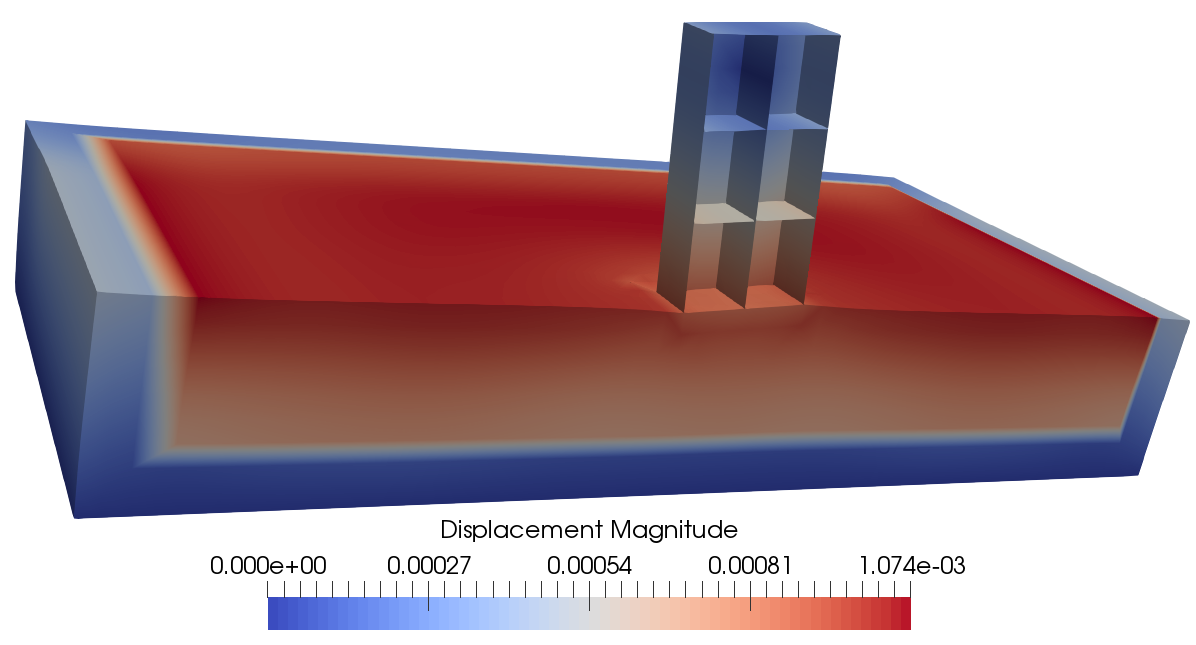
\includegraphics[width = 10cm]{./Figure-files/Day2/Deconvolution_1D_Motions/Shell_Structure_Soil_Interaction_3D_DRM/shell_DRM3D.png}
  \caption{Simulation Model}
  \label{fig_decon_1D_motion_3D_model_solid_shell_structure}
\end{figure}



























% ******************************************************************
% ******************************************************************
% ******************************************************************
\clearpage
\newpage
\section{Deconvolution 3$\times$1D Motions}
\label{Deconvolution_3by1D_Motions}
\subsection{Free field 1D model, deconvolution  3$\times$1D motion, model with DRM}
\label{Free_fields_1D_model_with_DRM2}

The Real-ESSI input files for this example are available 
\href{http://sokocalo.engr.ucdavis.edu/~jeremic/lecture_notes_online_material/_Chapter_Short_Course_Examples/Day2/Deconvolution_3by1D_Motions/Free_fields_1D_model_with_DRM}{HERE}. 
The compressed package of Real-ESSI input files for this example is available 
\href{http://sokocalo.engr.ucdavis.edu/~jeremic/lecture_notes_online_material/_Chapter_Short_Course_Examples/Day2/Deconvolution_3by1D_Motions/Free_fields_1D_model_with_DRM/_all_files_packaged_for_Free_fields_1D_model_with_DRM.tar.gz}{HERE}. 

The Modeling parameters are listed.
\begin{itemize}
  \item Elastic Material Properties 
  \begin{itemize}
    \item Mass density, $\rho$, \enspace \enspace 2000 $kg/m^3$
    \item Shear Wave Velocity, $V_s$, \enspace \enspace 500 $m/s$
    \item Young's modulus, $E$, \enspace \enspace 1.1 GPa
    \item Poisson's ratio, $\nu$, \enspace \enspace 0.1
  \end{itemize}
\end{itemize}

\begin{figure}[H]
  \centering
  \includegraphics[width = 0.8cm]{./Figure-files/Day2/Deconvolution_3by1D_Motions/Free_fields_1D_model_with_DRM/overview.png}
  \caption{Simulation Model}
  \label{fig_decon_1D_motion_1D_model2}
\end{figure}

The illustration results of the simulation is shown in Fig.~\ref{fig_decon_1D_motion_1D_model}.
As shown in the results, outside the DRM layer, there is no outgoing waves. 

\begin{figure}[H]
  \centering
  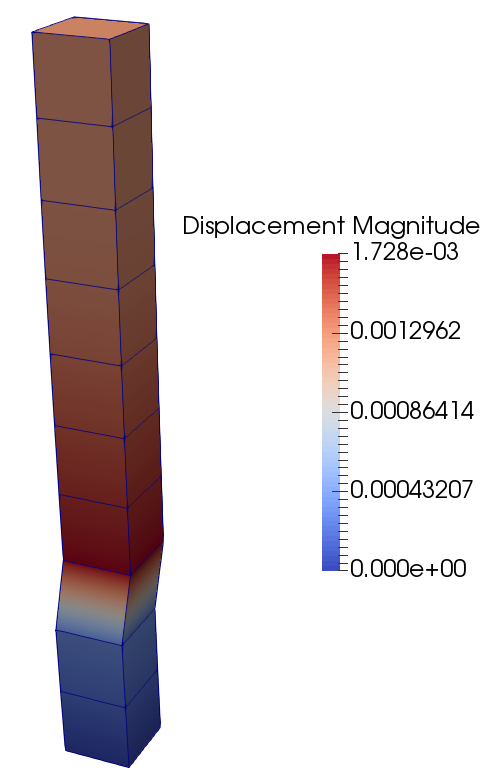
\includegraphics[width = 7cm]{./Figure-files/Day2/Deconvolution_3by1D_Motions/Free_fields_1D_model_with_DRM/DRM1D_Motion3D.png}
  \caption{Simulation Model}
  \label{fig_decon_3D_motion_1D_model_results}
\end{figure}


% ******************************************************************
% ******************************************************************
% ******************************************************************
\clearpage
\newpage
\subsection{Free field 3D model, deconvolution  3$\times$1D motion, model with DRM}
\label{Free_fields_3D_model_with_DRM2}

The Real-ESSI input files for this example are available 
\href{http://sokocalo.engr.ucdavis.edu/~jeremic/lecture_notes_online_material/_Chapter_Short_Course_Examples/Day2/Deconvolution_3by1D_Motions/Free_fields_3D_model_with_DRM}{HERE}. 
The compressed package of Real-ESSI input files for this example is available 
\href{http://sokocalo.engr.ucdavis.edu/~jeremic/lecture_notes_online_material/_Chapter_Short_Course_Examples/Day2/Deconvolution_3by1D_Motions/Free_fields_3D_model_with_DRM/_all_files_packaged_for_Free_fields_3D_model_with_DRM.tar.gz}{HERE}. 

The Modeling parameters are listed.
\begin{itemize}
  \item Elastic Soil Material Properties 
  \begin{itemize}
    \item Mass density, $\rho$, \enspace \enspace 2000 $kg/m^3$
    \item Shear Wave Velocity, $V_s$, \enspace \enspace 500 $m/s$
    \item Young's modulus, $E$, \enspace \enspace 1.1 GPa
    \item Poisson's ratio, $\nu$, \enspace \enspace 0.1
  \end{itemize}
\end{itemize}


\begin{figure}[H]
  \centering
  \includegraphics[width = 8cm]{./Figure-files/Day2/Deconvolution_3by1D_Motions/Free_fields_3D_model_with_DRM/overview.png}
  \caption{Simulation Model}
  \label{fig_decon_3by1D_motion_3D_model}
\end{figure}

The illustration results of the simulation is shown in Fig.~\ref{fig_decon_3D_motion_3D_model_results_free_field}.
As shown in the results, outside the DRM layer, there is no outgoing waves. 

\begin{figure}[H]
  \centering
  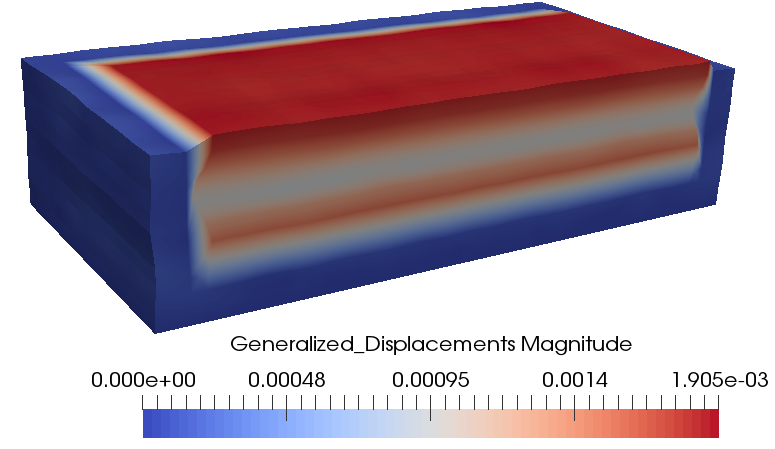
\includegraphics[width = 10cm]{./Figure-files/Day2/Deconvolution_3by1D_Motions/Free_fields_3D_model_with_DRM/motion3D_DRM3D_free_field.png}
  \caption{Simulation Model}
  \label{fig_decon_3D_motion_3D_model_results_free_field}
\end{figure}


% % ******************************************************************
% % ******************************************************************
% % ******************************************************************
% \clearpage
% \newpage
% \subsection{Free field 3D model, deconvolution  3$\times$1D motion, solid model with DRM}
% \label{Earthquake_Soil-structure_interaction_3D_model_with_DRM3}

% The Real-ESSI input files for this example are available 
% \href{http://sokocalo.engr.ucdavis.edu/~jeremic/lecture_notes_online_material/_Chapter_Short_Course_Examples/Day2/Deconvolution_3by1D_Motions/Earthquake_Soil-Structure_Interaction_3D_Model_with_DRM}{HERE}. 
% The compressed package of Real-ESSI input files for this example is available 
% \href{http://sokocalo.engr.ucdavis.edu/~jeremic/lecture_notes_online_material/_Chapter_Short_Course_Examples/Day2/Deconvolution_3by1D_Motions/Earthquake_Soil-Structure_Interaction_3D_Model_with_DRM/_all_files_packaged_for_Earthquake_Soil-Structure_Interaction_3D_Model_with_DRM.tar.gz}{HERE}. 

% The Modeling parameters are listed.
% \begin{itemize}
%   \item Elastic Soil Material Properties 
%   \begin{itemize}
%     \item Mass density, $\rho$, \enspace \enspace 2000 $kg/m^3$
%     \item Shear Wave Velocity, $V_s$, \enspace \enspace 500 $m/s$
%     \item Young's modulus, $E$, \enspace \enspace 1.1 GPa
%     \item Poisson's ratio, $\nu$, \enspace \enspace 0.1
%   \end{itemize}
%   \item Elastic Structure Material Properties 
%   \begin{itemize}
%     \item Mass density, $\rho$, \enspace \enspace 2500 $kg/m^3$
%     \item Young's modulus, $E$, \enspace \enspace 20 GPa
%     \item Poisson's ratio, $\nu$, \enspace \enspace 0.1
%   \end{itemize}
% \end{itemize}

% \begin{figure}[H]
%   \centering
%   \includegraphics[width = 8cm]{./Figure-files/Day2/Deconvolution_3by1D_Motions/Earthquake_Soil-Structure_Interaction_3D_Model_with_DRM/overview.png}
%   \caption{Simulation Model}
%   \label{fig_decon_1D_motion_3D_model3}
% \end{figure}


% The illustration results of the simulation is shown in Fig.~\ref{fig_decon_3D_motion_3D_model_results_structure}.
% As shown in the results, outside the DRM layer, there is no outgoing waves. 

% \begin{figure}[H]
%   \centering
%   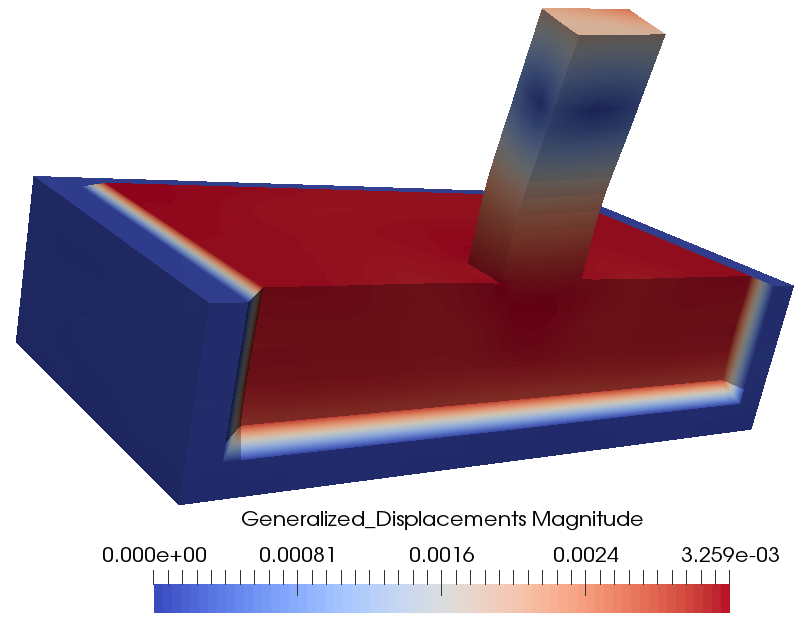
\includegraphics[width = 10cm]{./Figure-files/Day2/Deconvolution_3by1D_Motions/Earthquake_Soil-Structure_Interaction_3D_Model_with_DRM/DRM3D_motion3D_structure.png}
%   \caption{Simulation Model}
%   \label{fig_decon_3D_motion_3D_model_results_structure}
% \end{figure}





% ******************************************************************
% ******************************************************************
% ******************************************************************
\clearpage
\newpage
\subsection{ESSI 3D building model, deconvolution  3$\times$1D motion, shell model with DRM}
\label{Earthquake_Soil-Structure_Interaction_3D_Model_with_DRM4}

The Real-ESSI input files for this example are available 
\href{http://sokocalo.engr.ucdavis.edu/~jeremic/lecture_notes_online_material/_Chapter_Short_Course_Examples/Day2/Deconvolution_3by1D_Motions/Shell_Structure_Soil_Interaction_3D_DRM}{HERE}. 
The compressed package of Real-ESSI input files for this example is available 
\href{http://sokocalo.engr.ucdavis.edu/~jeremic/lecture_notes_online_material/_Chapter_Short_Course_Examples/Day2/Deconvolution_3by1D_Motions/Shell_Structure_Soil_Interaction_3D_DRM/_all_files_packaged_for_Shell_Structure_Soil_Interaction_3D_DRM.tar.gz}{HERE}. 

The Modeling parameters are listed.
\begin{itemize}
  \item Elastic Soil Material Properties 
  \begin{itemize}
    \item Mass density, $\rho$, \enspace \enspace 2000 $kg/m^3$
    \item Shear Wave Velocity, $V_s$, \enspace \enspace 500 $m/s$
    \item Young's modulus, $E$, \enspace \enspace 1.1 GPa
    \item Poisson's ratio, $\nu$, \enspace \enspace 0.1
  \end{itemize}
  \item Elastic Structure Material Properties 
  \begin{itemize}
    \item Mass density, $\rho$, \enspace \enspace 2500 $kg/m^3$
    \item Young's modulus, $E$, \enspace \enspace 20 GPa
    \item Poisson's ratio, $\nu$, \enspace \enspace 0.1
  \end{itemize}
\end{itemize}

\begin{figure}[H]
  \centering
  \includegraphics[width = 8cm]{./Figure-files/Day2/Deconvolution_3by1D_Motions/Shell_Structure_Soil_Interaction_3D_DRM/overview.png}
  \caption{Simulation Model}
  \label{fig_decon_3by1D_motion_3D_model_shell}
\end{figure}


The illustration results of DRM 3D shell Structure Model under 1D motion is shown 
in Fig.~\ref{fig_decon_3by1D_motion_3D_model_solid_shell_structure}. 

\begin{figure}[H]
  \centering
  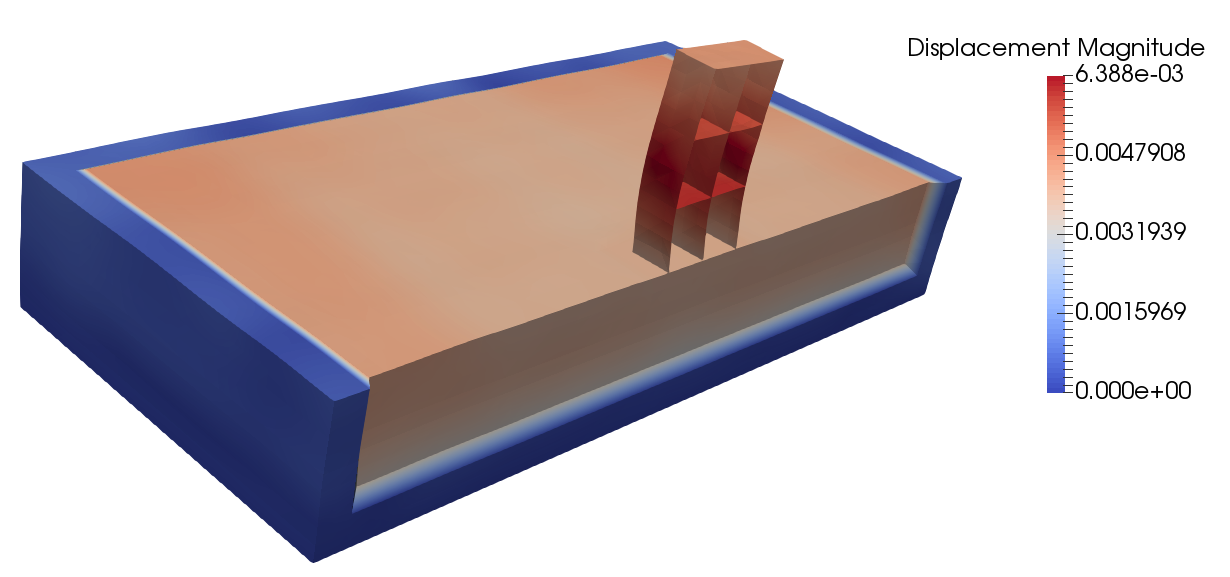
\includegraphics[width = 10cm]{./Figure-files/Day2/Deconvolution_3by1D_Motions/Shell_Structure_Soil_Interaction_3D_DRM/DRM3D_motion3D_shell.png}
  \caption{Simulation Model}
  \label{fig_decon_3by1D_motion_3D_model_solid_shell_structure}
\end{figure}


















% ******************************************************************
% ******************************************************************
% ******************************************************************
\clearpage
\newpage
\section{Mesh Dependence of Wave Propagation Frequencies}
\label{Convolution_Motions}


The Real-ESSI input files for this example are available 
\href{http://sokocalo.engr.ucdavis.edu/~jeremic/lecture_notes_online_material/_Chapter_Short_Course_Examples/Day2/Convolution_Motions}{HERE}. 
The compressed package of Real-ESSI input files for this example is available 
\href{http://sokocalo.engr.ucdavis.edu/~jeremic/lecture_notes_online_material/_Chapter_Short_Course_Examples/Day2/Convolution_Motions/_all_files_packaged_for_Convolution_Motions.tar.gz}{HERE}. 


Show the mesh dependence of high frequency wave with Ormsby wavelet.

\begin{figure}[H]
  \centering
  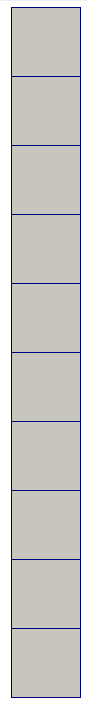
\includegraphics[width = 0.5cm]{./Figure-files/Day2/Convolution_Motions/overview.png}
  \caption{Simulation Model}
  \label{fig_decon_1D_motion_3D_model4}
\end{figure}

The illustration results of mesh dependence is shown in Fig.~\ref{fig_day2_convolution_time_freq}.

\begin{figure}[H]
  \centering
  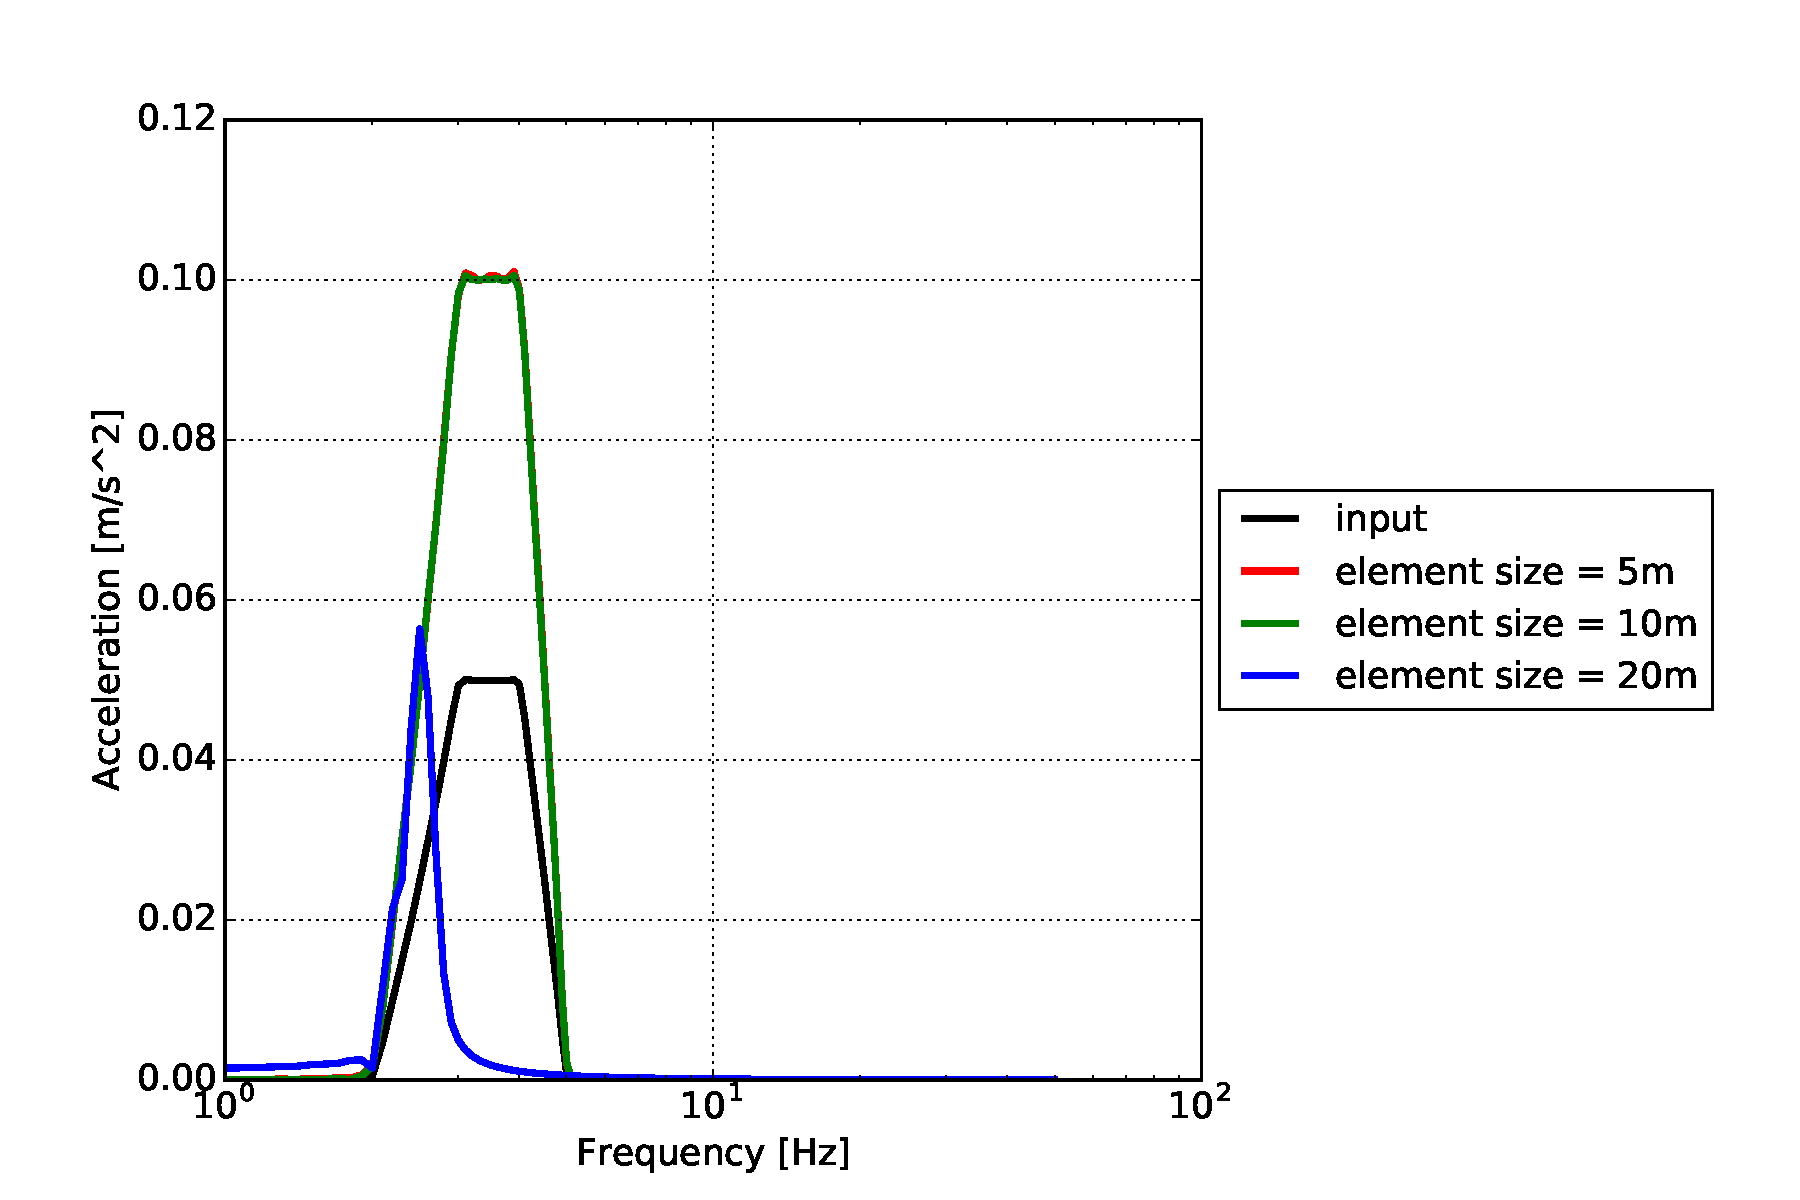
\includegraphics[width = 12cm]{./Figure-files/Day2/Convolution_Motions/top_acc_feq_all.pdf}
  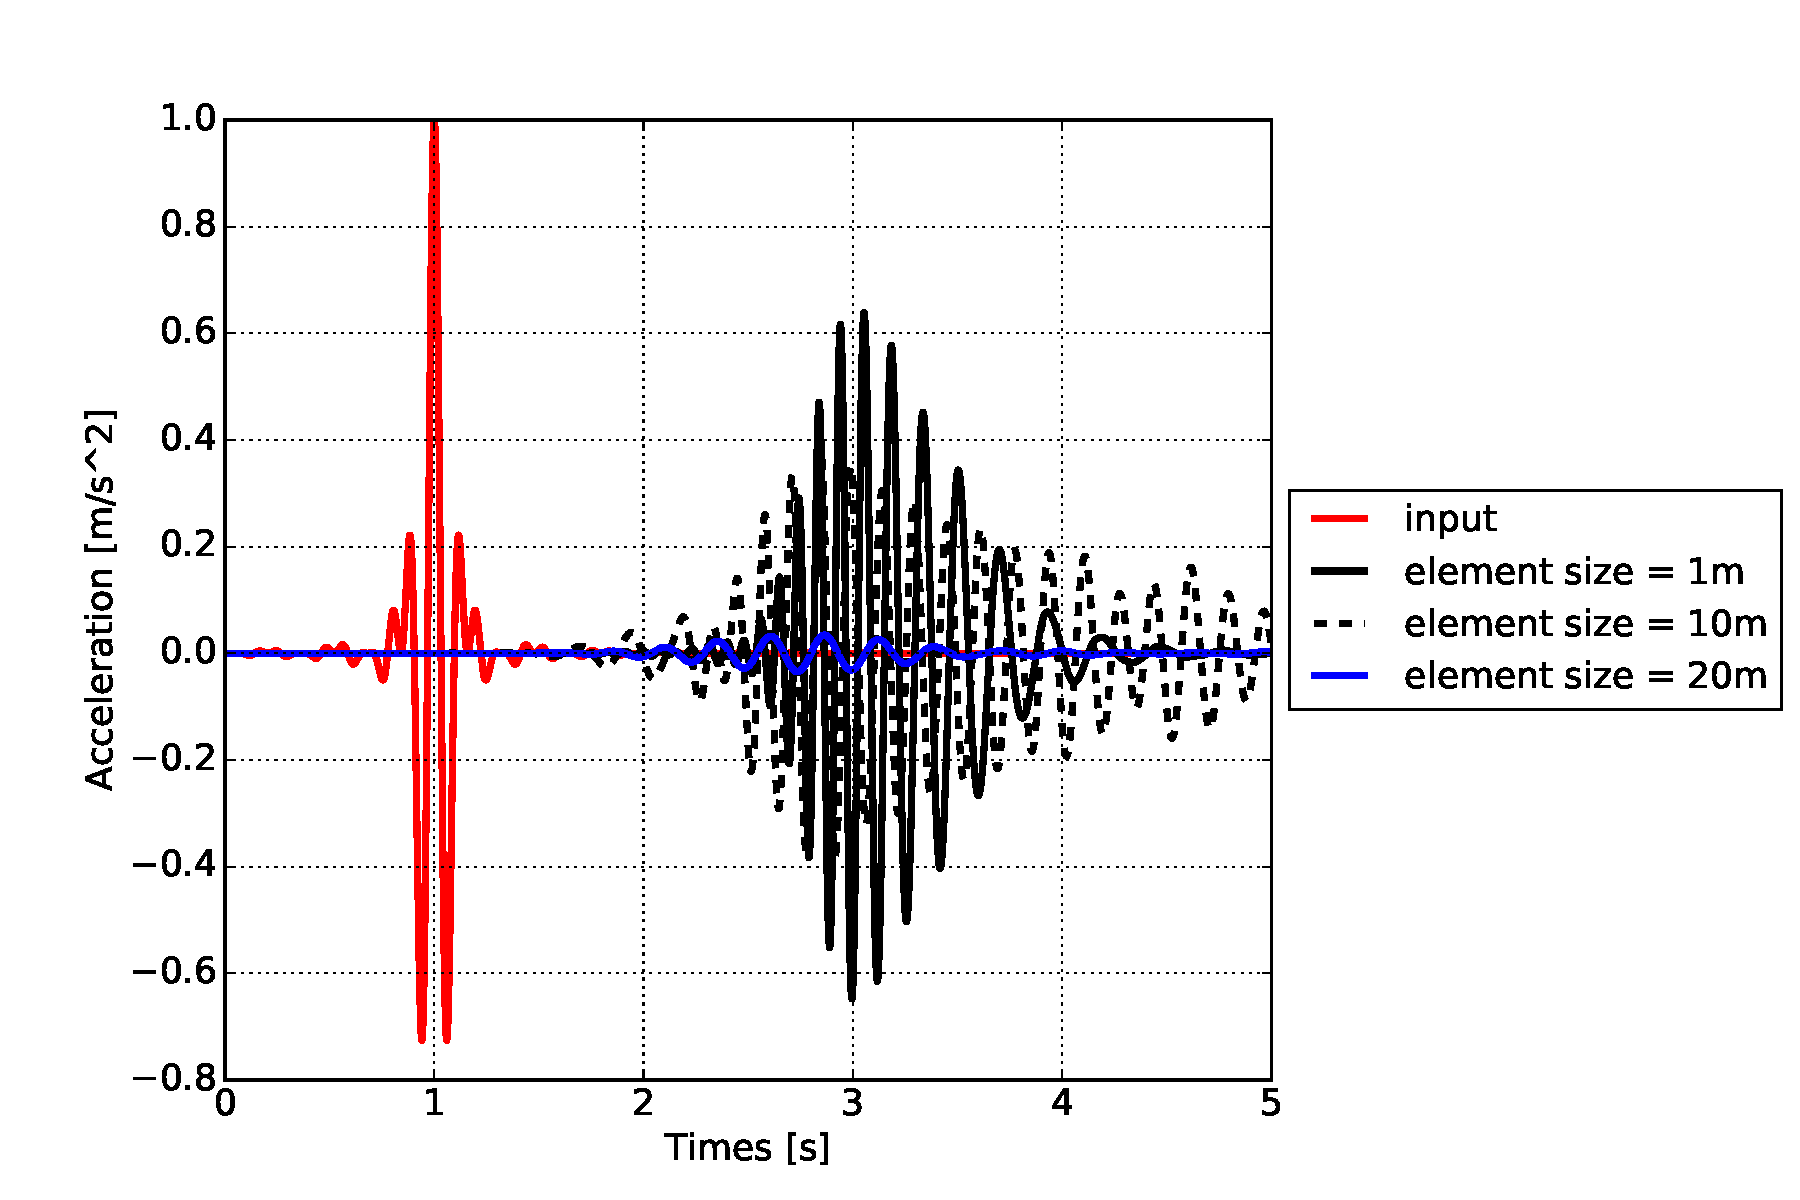
\includegraphics[width = 12cm]{./Figure-files/Day2/Convolution_Motions/top_acc_time_all.pdf}
  \caption{Convolution Results and Mesh Dependence}
  \label{fig_day2_convolution_time_freq}
\end{figure}



































% ******************************************************************
% ******************************************************************
% ******************************************************************
\clearpage
\newpage
\section{Apply 3D Motions from SW4}
\label{Apply_3D_Motions_from_SW4}

\subsection{3D seismic motion by SW4}
\label{3D seismic motion by SW4}

A 3D seismic motion field has been developed by SW4. The characteristic parameters of the seismic motion are given below: 

\begin{itemize}
  \item Geological model:  length $3km$, width 3$km$, height $1.7km$, grid size $50m$, width of super grid damping layer $30m$.  
  \item Material model: Elastic material, First $1km$: $V_p= 4630.76m/s$, $V_s=2437.56m/s$, $\rho = 2600kg/m^3$.  $1km\sim1.7km$: $V_p=6000m/s$, $V_s=3464m/s$, $\rho = 2700kg/m^3$ 
  \item Source type: point moment source, moment seismic moment $M_{xy} = 5e^{15} N \cdot m$, moment magnitude 4.5. 
  \item Time function: Gaussian function, with dominant frequency $2.5Hz$ and maximum frequency $6.5Hz$. 
\end{itemize}  

The time series displacement and acceleration response at the center of the model is shown below in figure \ref{3D_motion_time_response}. 
%
And figure \ref{3D_motion_fft_response} gives corresponding FFT response. 

\begin{figure}[H]
  \centering
  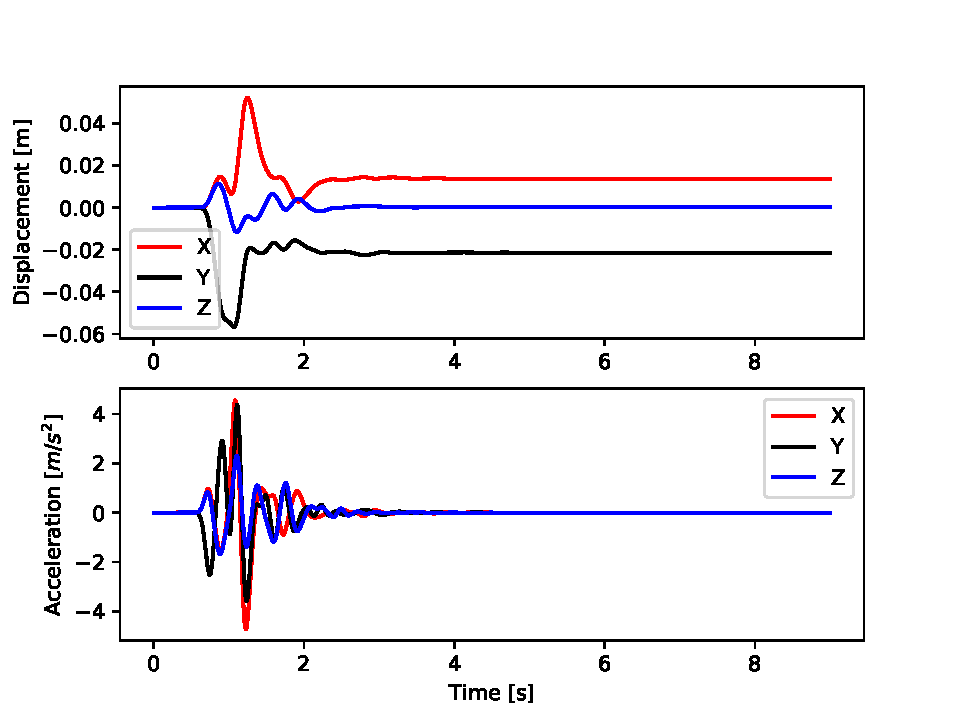
\includegraphics[width = 8cm]{./Figure-files/Day2/Apply_3D_Motions_from_SW4/3D_seismic_motion_by_SW4/time_response.pdf}
  \caption{Time series response of 3D motion}
  \label{3D_motion_time_response}
\end{figure}

\begin{figure}[H]
  \centering
  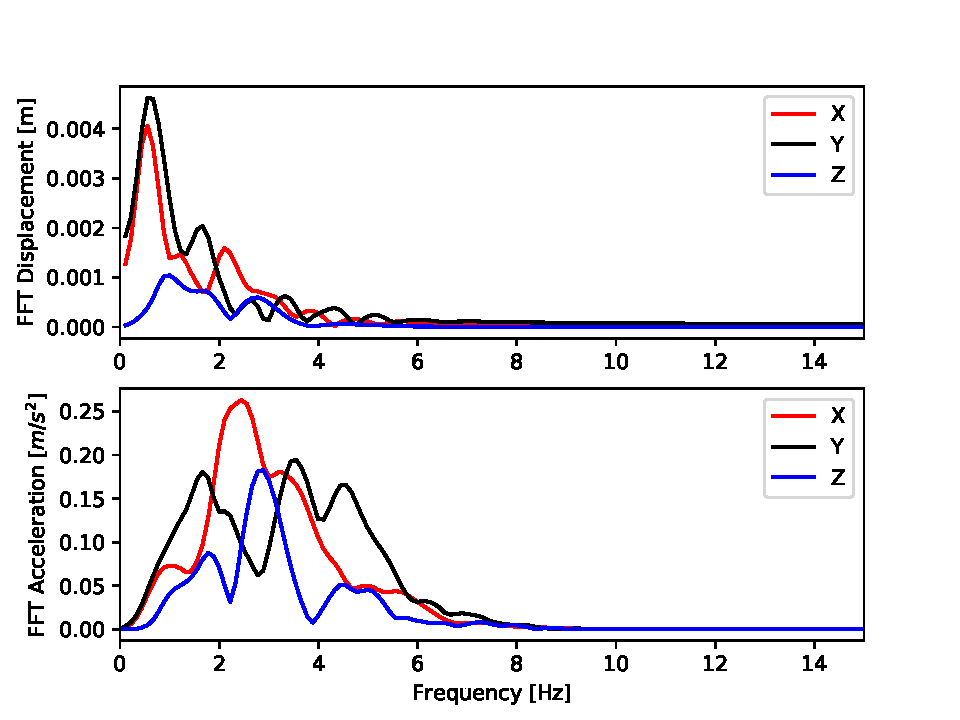
\includegraphics[width = 8cm]{./Figure-files/Day2/Apply_3D_Motions_from_SW4/3D_seismic_motion_by_SW4/frequency_response.pdf}
  \caption{FFT response of 3D motion}
  \label{3D_motion_fft_response}
\end{figure}

During the simulation of SW4, the time series motions at many ESSI nodes (basically are some pre-defined record stations) of an ESSI box ($300m\times300m\times100m$) are recorded and written into \textbf{SAC} files. 
%
Then an transition program SW42ESSI has been developed to interpolate these motions to DRM nodes of localized ESSI model by specifying some geometric translational and rotational transformation, as shown in figure \ref{Transition from SW4 to Real ESSI}. 
%

To launch SW42ESSI, following parameters are needed: 

\begin{itemize}

  \item DRM input: specify the name of DRM input files. This DRM file just contains the geometric information of DRM layer in ESSI model (e.g. DRM node IDs, nodal coordinates, etc). 

  \item SW4 motion directory: specify the output directory of SW4, that contains SAC files. 

  \item origin coordinates of ESSI box (x, y, z): the SW4 coordinates of the origin of ESSI box, i.e. the coordinates of ESSI nodes, whose station ID is (0, 0, 0). 

  \item dimensions of ESSI Box (length, width, height): specify the dimension (length, width and height) of ESSI box. 

  \item spacing of ESSI nodes: specify the grid spacing of ESSI nodes (i.e. motion recording stations)

  \item interval of time steps for sampling: specify the sampling frequency, if 1 is used here, ESSI simulation time step is the same as the simulation time step of SW4.   

  \item reference point in ESSI model for translational transformation (x, y, z): specify the coordinate of reference point for translational transformation in ESSI model. 

  \item reference point in SW4 model for translational transformation (x, y, z): specify the coordinate of reference point for translational transformation in SW4 model. 

  \item conduct rotational transformation (yes/no): input yes and provide more rotational transformation parameters to enable rotational transformation. If input no, no more parameters are required.  

  \item reference point in SW4 model for rotational transformation (x, y, z): specify the coordinate of reference point for rotational transformation in SW4 model. 

  \item degrees of rotation along three axes (x, y, z): specify the degrees of rotation along three axes. The sign of rotation degrees follows right hand rule. 

\end{itemize}

\begin{figure}[H]
  \centering
  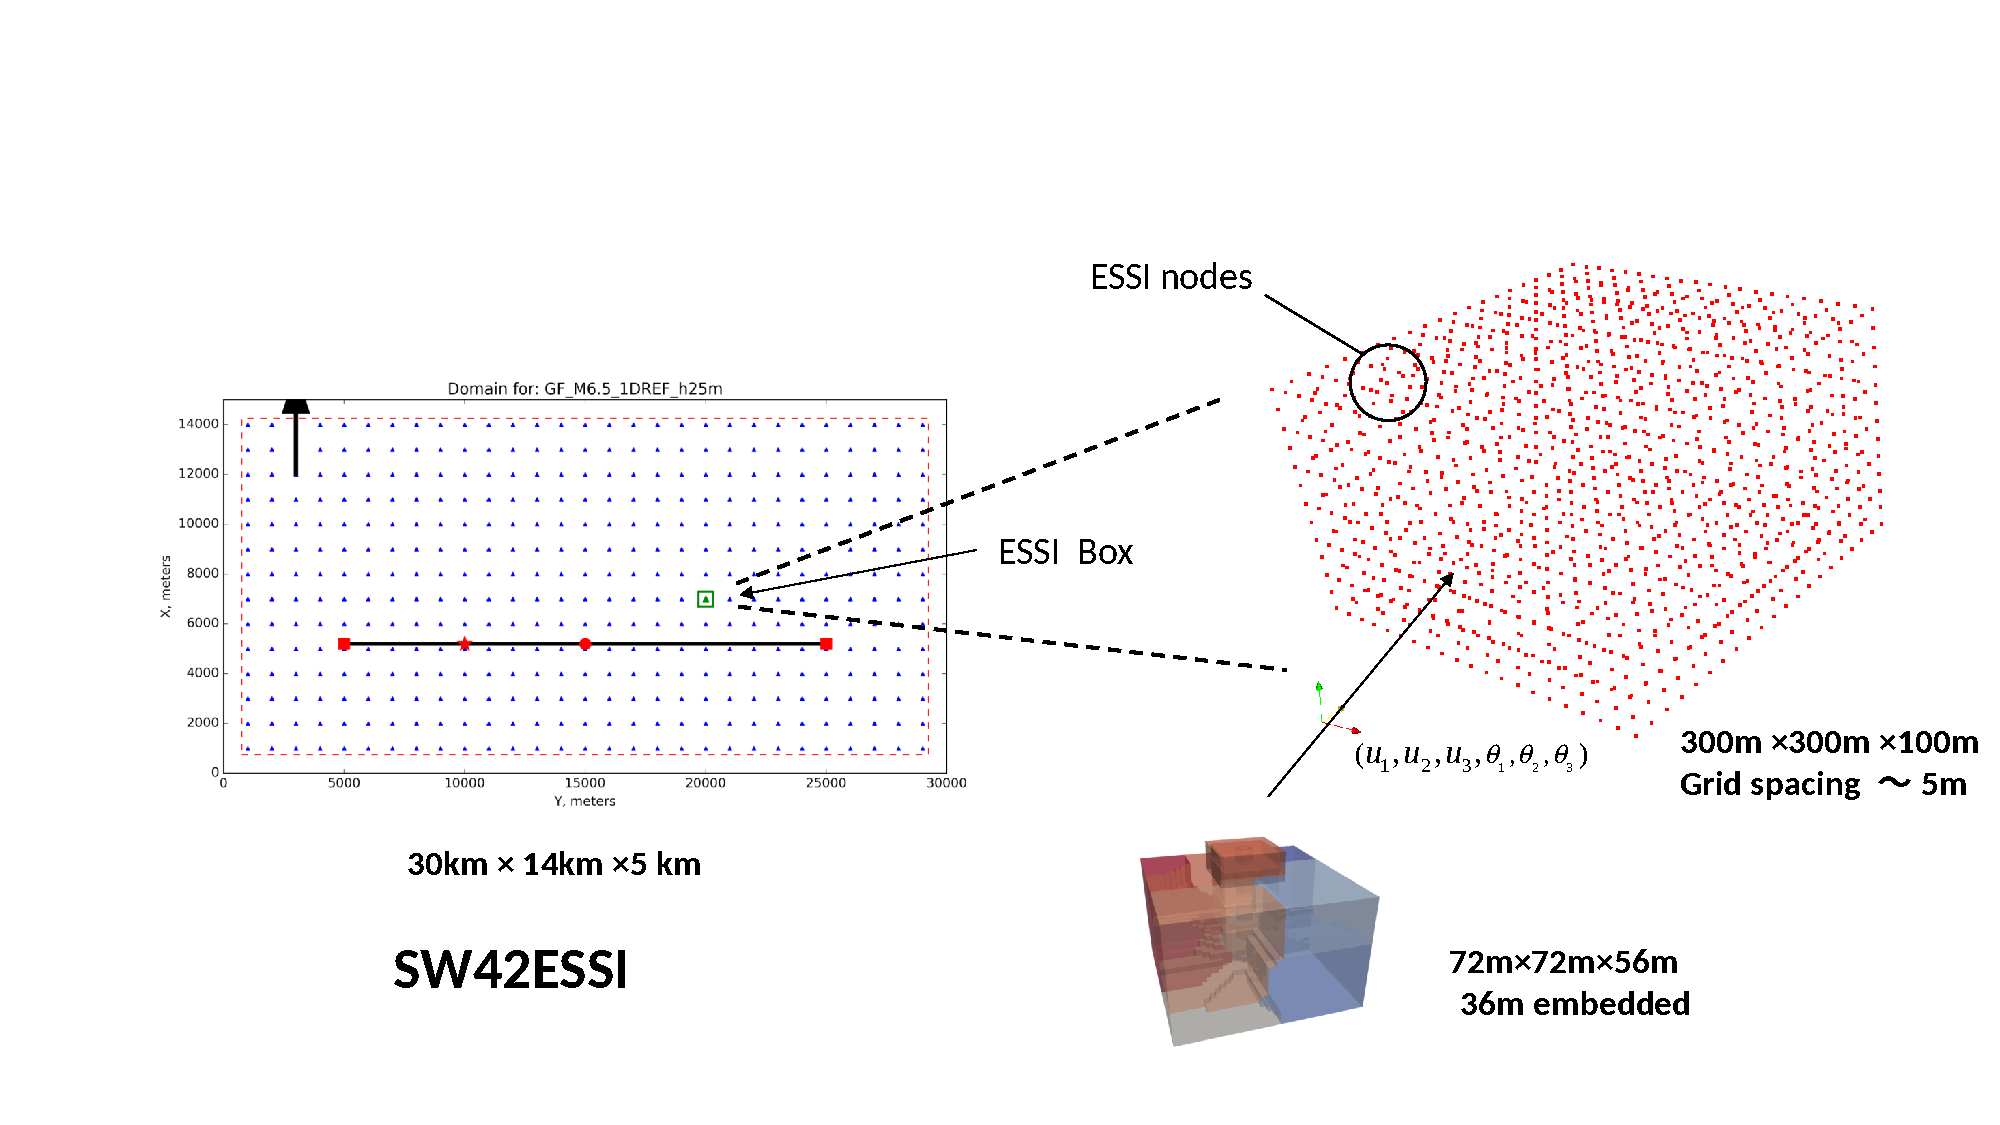
\includegraphics[width = \textwidth]{./Figure-files/Day2/Apply_3D_Motions_from_SW4/3D_seismic_motion_by_SW4/SW42DRM.pdf}
  \caption{Illustration of transition from SW4 to Real ESSI}
  \label{Transition from SW4 to Real ESSI}
\end{figure}


\subsection{Free field 3D model, 3D motion, model with DRM}
\label{Free_fields_3D_model_with_DRM3}


The Real-ESSI input files for this example are available 
\href{http://sokocalo.engr.ucdavis.edu/~jeremic/lecture_notes_online_material/_Chapter_Short_Course_Examples/Day2/Apply_3D_Motions_from_SW4/Free_fields_3D_model_with_DRM}{HERE}. 
The compressed package of Real-ESSI input files for this example is available 
\href{http://sokocalo.engr.ucdavis.edu/~jeremic/lecture_notes_online_material/_Chapter_Short_Course_Examples/Day2/Apply_3D_Motions_from_SW4/Free_fields_3D_model_with_DRM/_all_files_packaged_for_Free_fields_3D_model_with_DRM.tar.gz}{HERE}. 


\begin{figure}[H]
  \centering
  \includegraphics[width = 8cm]{./Figure-files/Day2/Apply_3D_Motions_from_SW4/Free_fields_3D_model_with_DRM/overview.png}
  \caption{Simulation Model}
  \label{fig_decon_1D_motion_3D_model5}
\end{figure}


The illustration results of free field DRM 3D Model under 3D motion is shown in figure \ref{3D_free_field_model_under_3D_motion}. 

\begin{figure}[H]
  \centering
  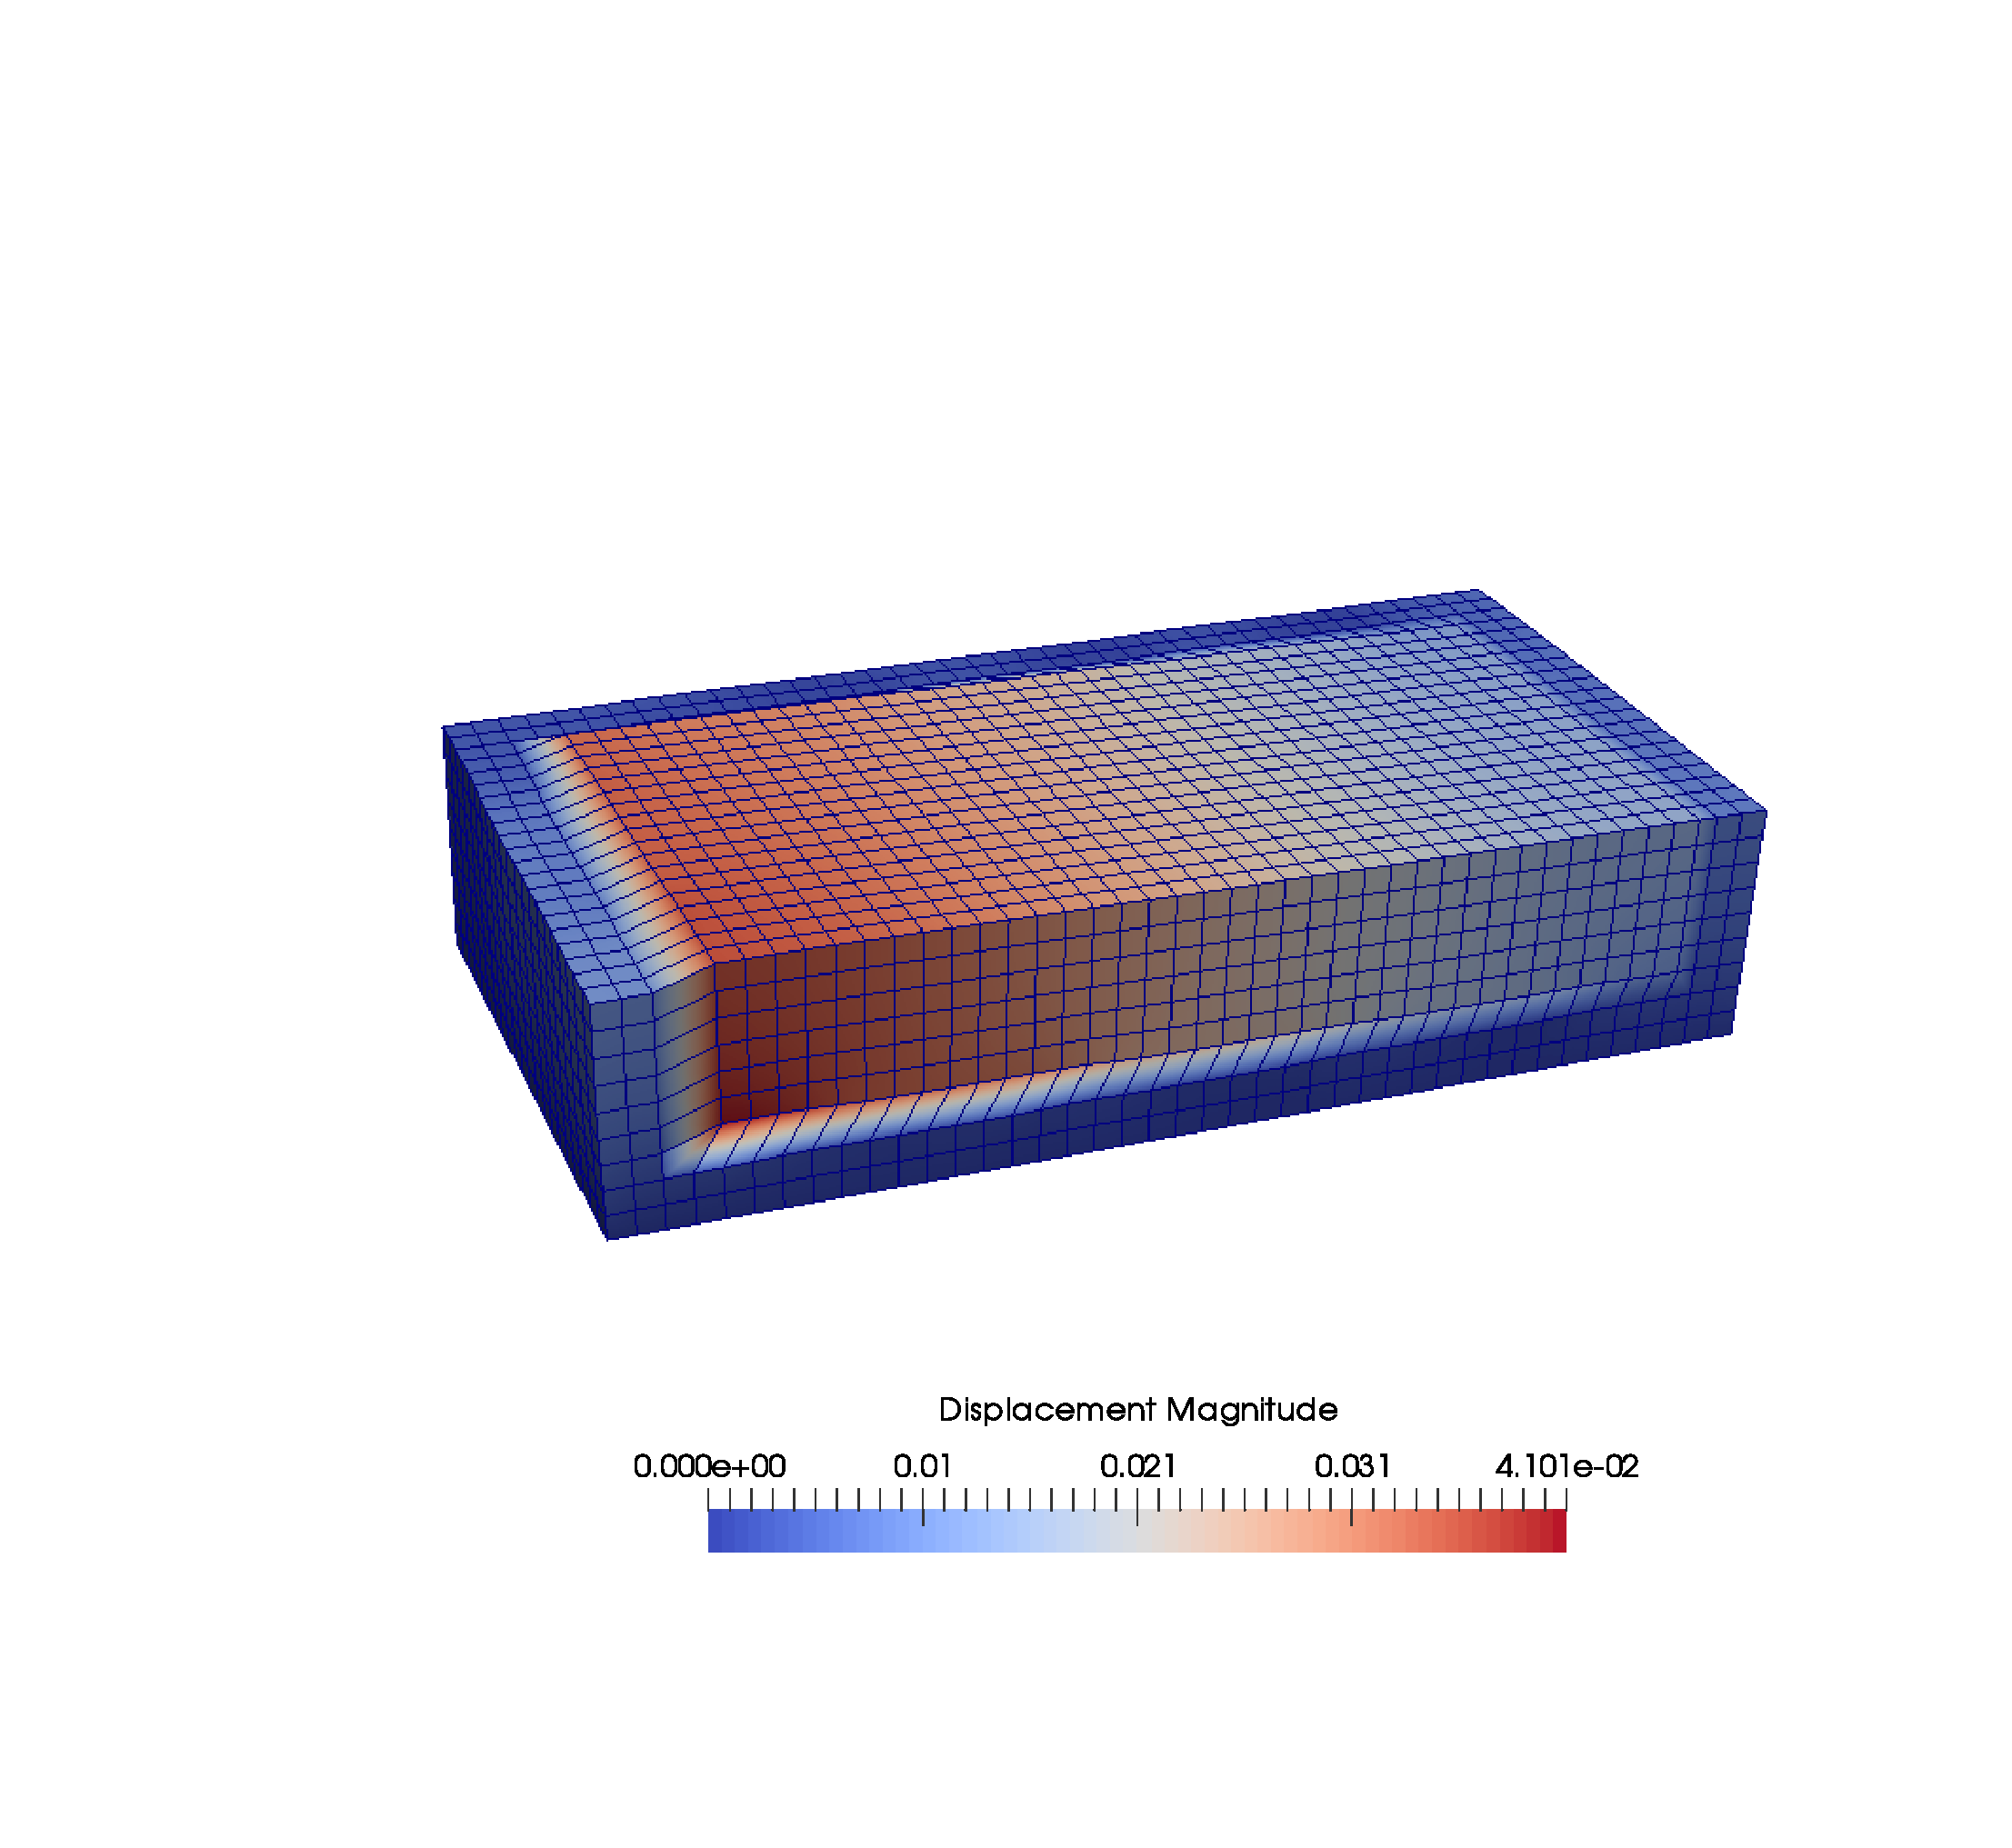
\includegraphics[width = 10cm]{./Figure-files/Day2/Apply_3D_Motions_from_SW4/Free_fields_3D_model_with_DRM/Free_field_model_3D_motion.pdf}
  \caption{Simulation of 3D free field model under 3D seismic motion}
  \label{3D_free_field_model_under_3D_motion}
\end{figure}



% % ******************************************************************
% % ******************************************************************
% % ******************************************************************
% \clearpage
% \newpage
% \subsection{ESSI 3D building model, 3D motion, solid model with DRM}
% \label{Earthquake_Soil-Structure_Interaction_3D_Model_with_DRM5}

% The Real-ESSI input files for this example are available 
% \href{http://sokocalo.engr.ucdavis.edu/~jeremic/lecture_notes_online_material/_Chapter_Short_Course_Examples/Day2/Apply_3D_Motions_from_SW4/Earthquake_Soil-Structure_Interaction_3D_Model_with_DRM}{HERE}. 
% The compressed package of Real-ESSI input files for this example is available 
% \href{http://sokocalo.engr.ucdavis.edu/~jeremic/lecture_notes_online_material/_Chapter_Short_Course_Examples/Day2/Apply_3D_Motions_from_SW4/Earthquake_Soil-Structure_Interaction_3D_Model_with_DRM/_all_files_packaged_for_Earthquake_Soil-Structure_Interaction_3D_Model_with_DRM.tar.gz}{HERE}. 


% \begin{figure}[H]
%   \centering
%   \includegraphics[width = 8cm]{./Figure-files/Day2/Apply_3D_Motions_from_SW4/Earthquake_Soil-Structure_Interaction_3D_Model_with_DRM/overview.png}
%   \caption{Simulation Model}
%   \label{fig_decon_1D_motion_3D_model6}
% \end{figure}


% The illustration results of DRM 3D Solid Structure Model  under 3D motion is shown in figure \ref{3D_solid_model_3D_seismic_motion}. 

% \begin{figure}[H]
%   \centering
%   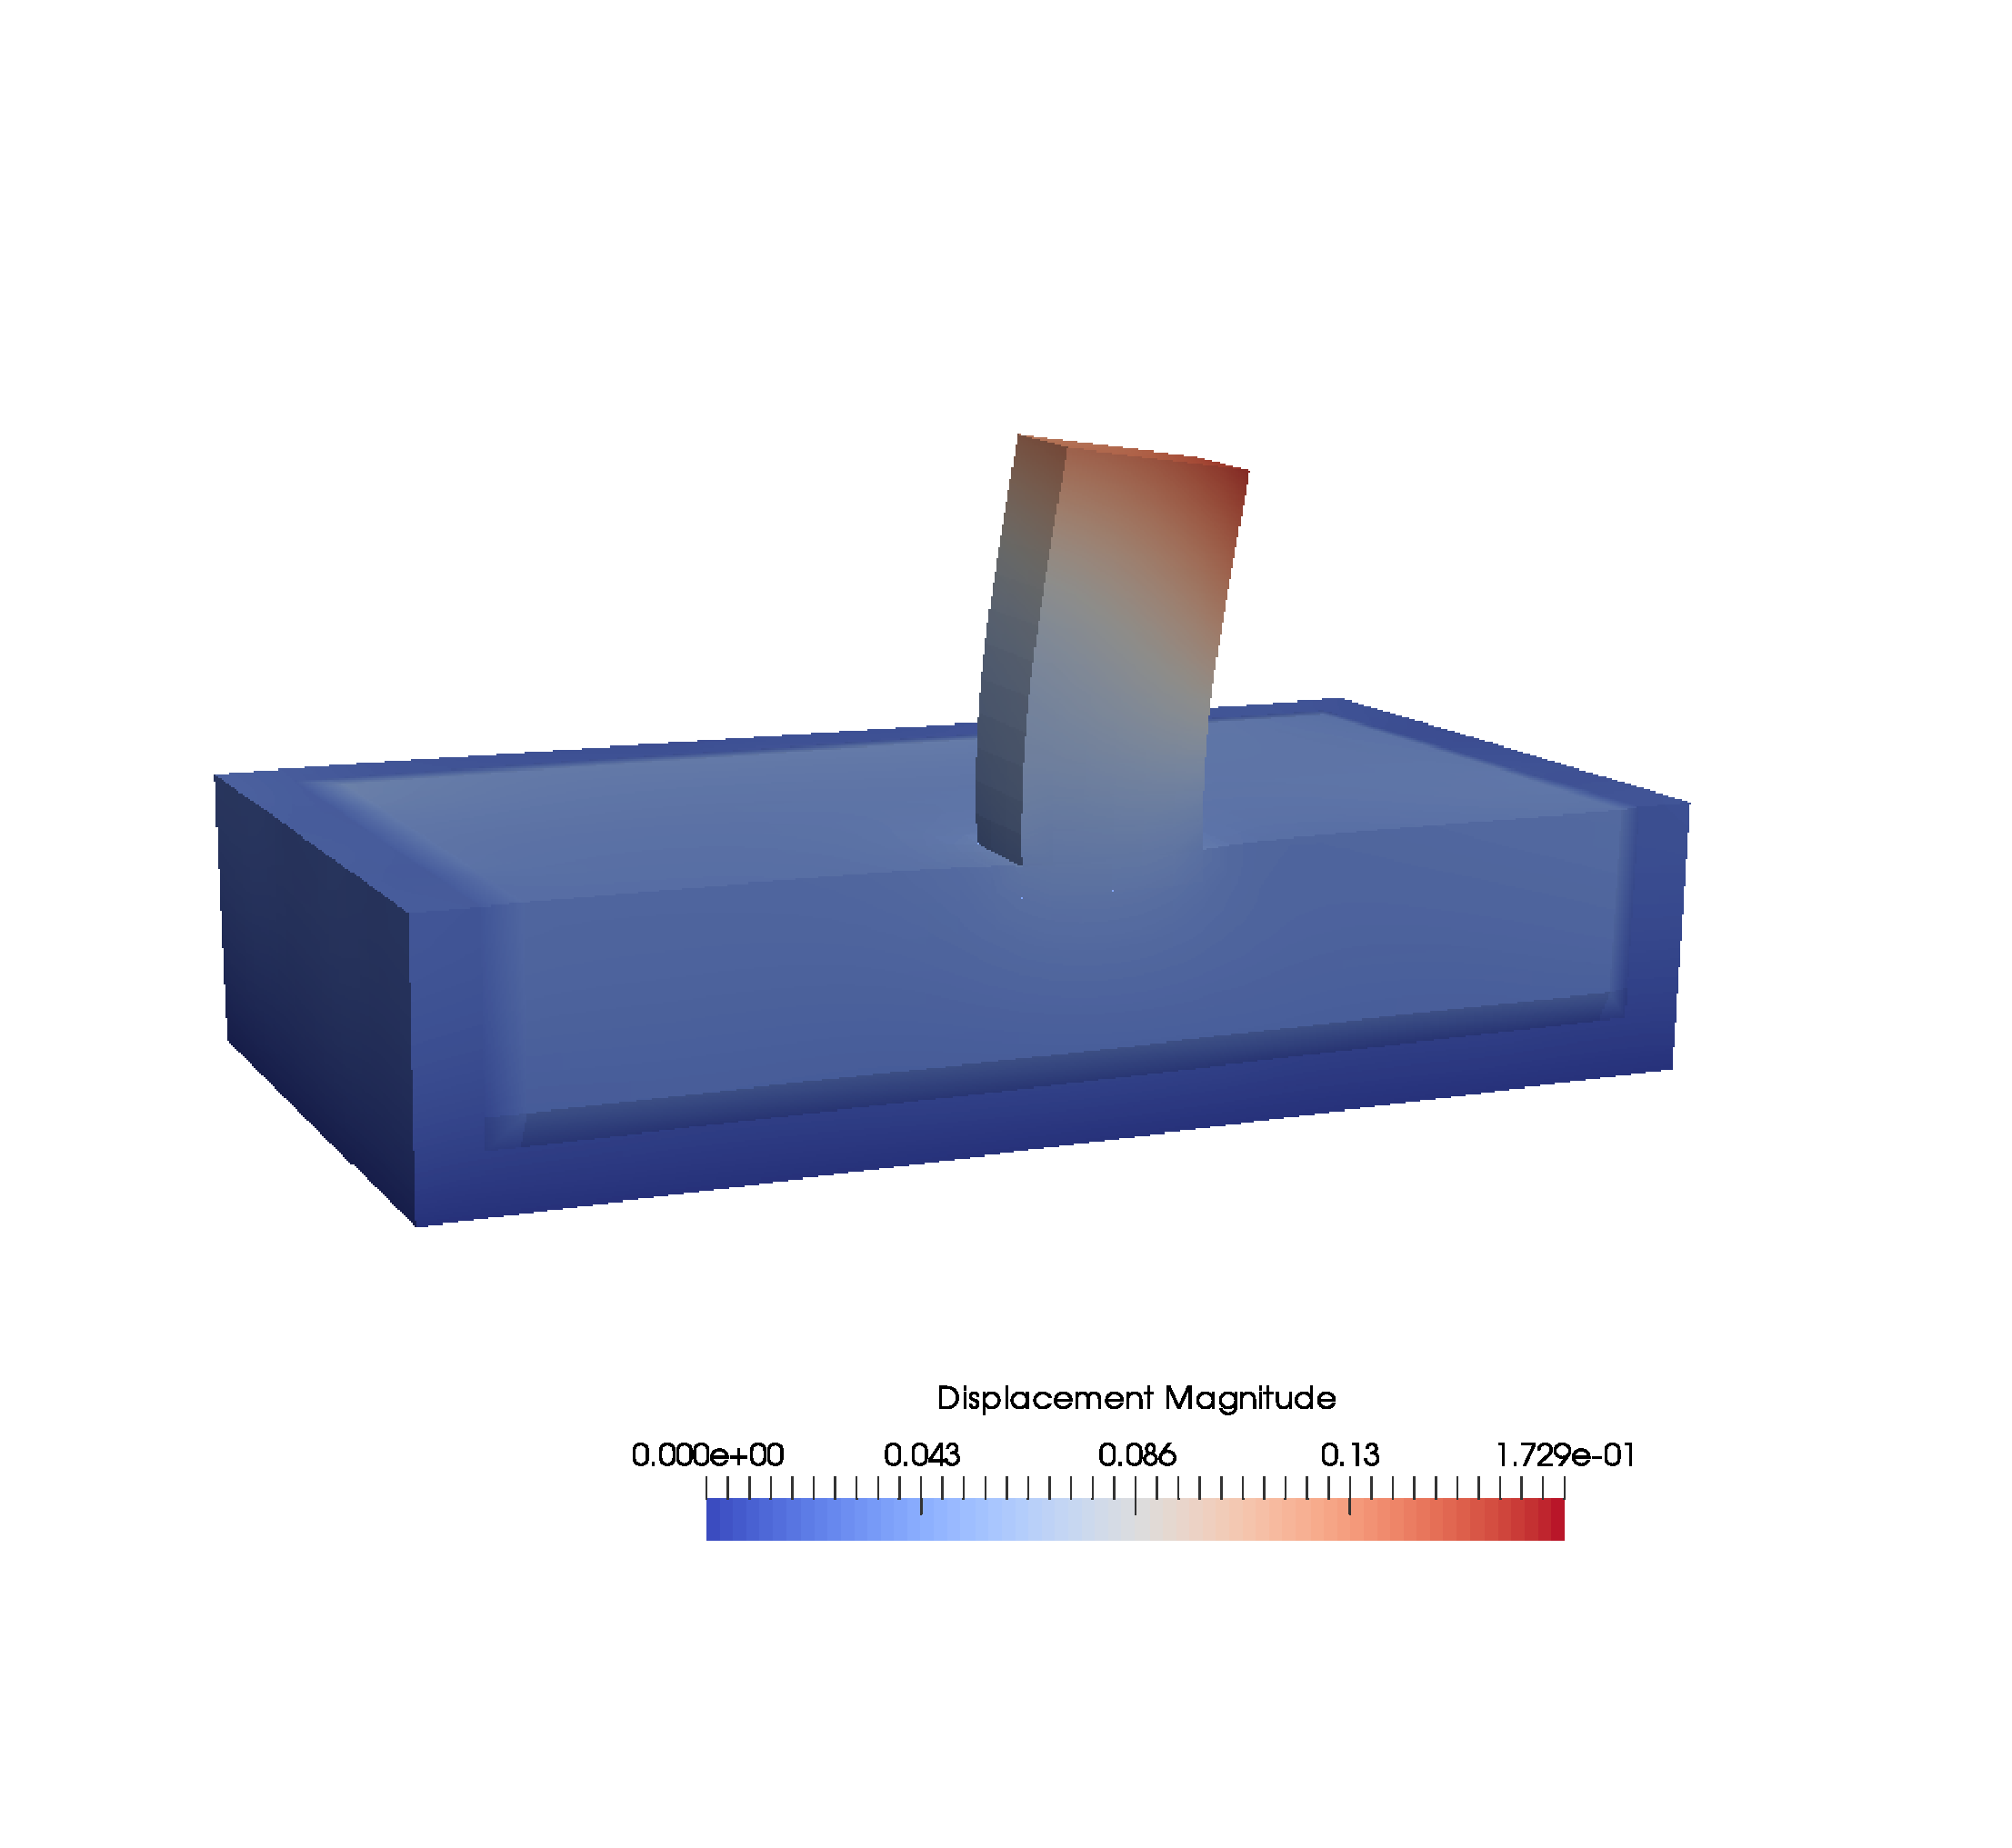
\includegraphics[width = 10cm]{./Figure-files/Day2/Apply_3D_Motions_from_SW4/Earthquake_Soil-Structure_Interaction_3D_Model_with_DRM/3D_solid_model_3D_motion.pdf}
%   \caption{Simulation of 3D solid model under 3D seismic motions}
%   \label{3D_solid_model_3D_seismic_motion}
% \end{figure}




% ******************************************************************
% ******************************************************************
% ******************************************************************
\clearpage
\newpage
\subsection{ESSI 3D building model, 3D motion, shell model with DRM}
\label{Earthquake_Soil-Structure_Interaction_3D_Model_with_DRM6}

The Real-ESSI input files for this example are available 
\href{http://sokocalo.engr.ucdavis.edu/~jeremic/lecture_notes_online_material/_Chapter_Short_Course_Examples/Day2/Apply_3D_Motions_from_SW4/Shell_Structure_Soil_Interaction_3D_DRM}{HERE}. 
The compressed package of Real-ESSI input files for this example is available 
\href{http://sokocalo.engr.ucdavis.edu/~jeremic/lecture_notes_online_material/_Chapter_Short_Course_Examples/Day2/Apply_3D_Motions_from_SW4/Shell_Structure_Soil_Interaction_3D_DRM/_all_files_packaged_for_Shell_Structure_Soil_Interaction_3D_DRM.tar.gz}{HERE}. 


\begin{figure}[H]
  \centering
  \includegraphics[width = 8cm]{./Figure-files/Day2/Apply_3D_Motions_from_SW4/Shell_Structure_Soil_Interaction_3D_DRM/overview.png}
  \caption{Simulation Model}
  \label{fig_decon_1D_motion_3D_model_shell2}
\end{figure}


% The illustration results of DRM 3D shell Structure Model under 3D seismic motion is shown in figure \ref{3D shell model under 3D seismic motion}. 

% \begin{figure}[H]
%   \centering
%   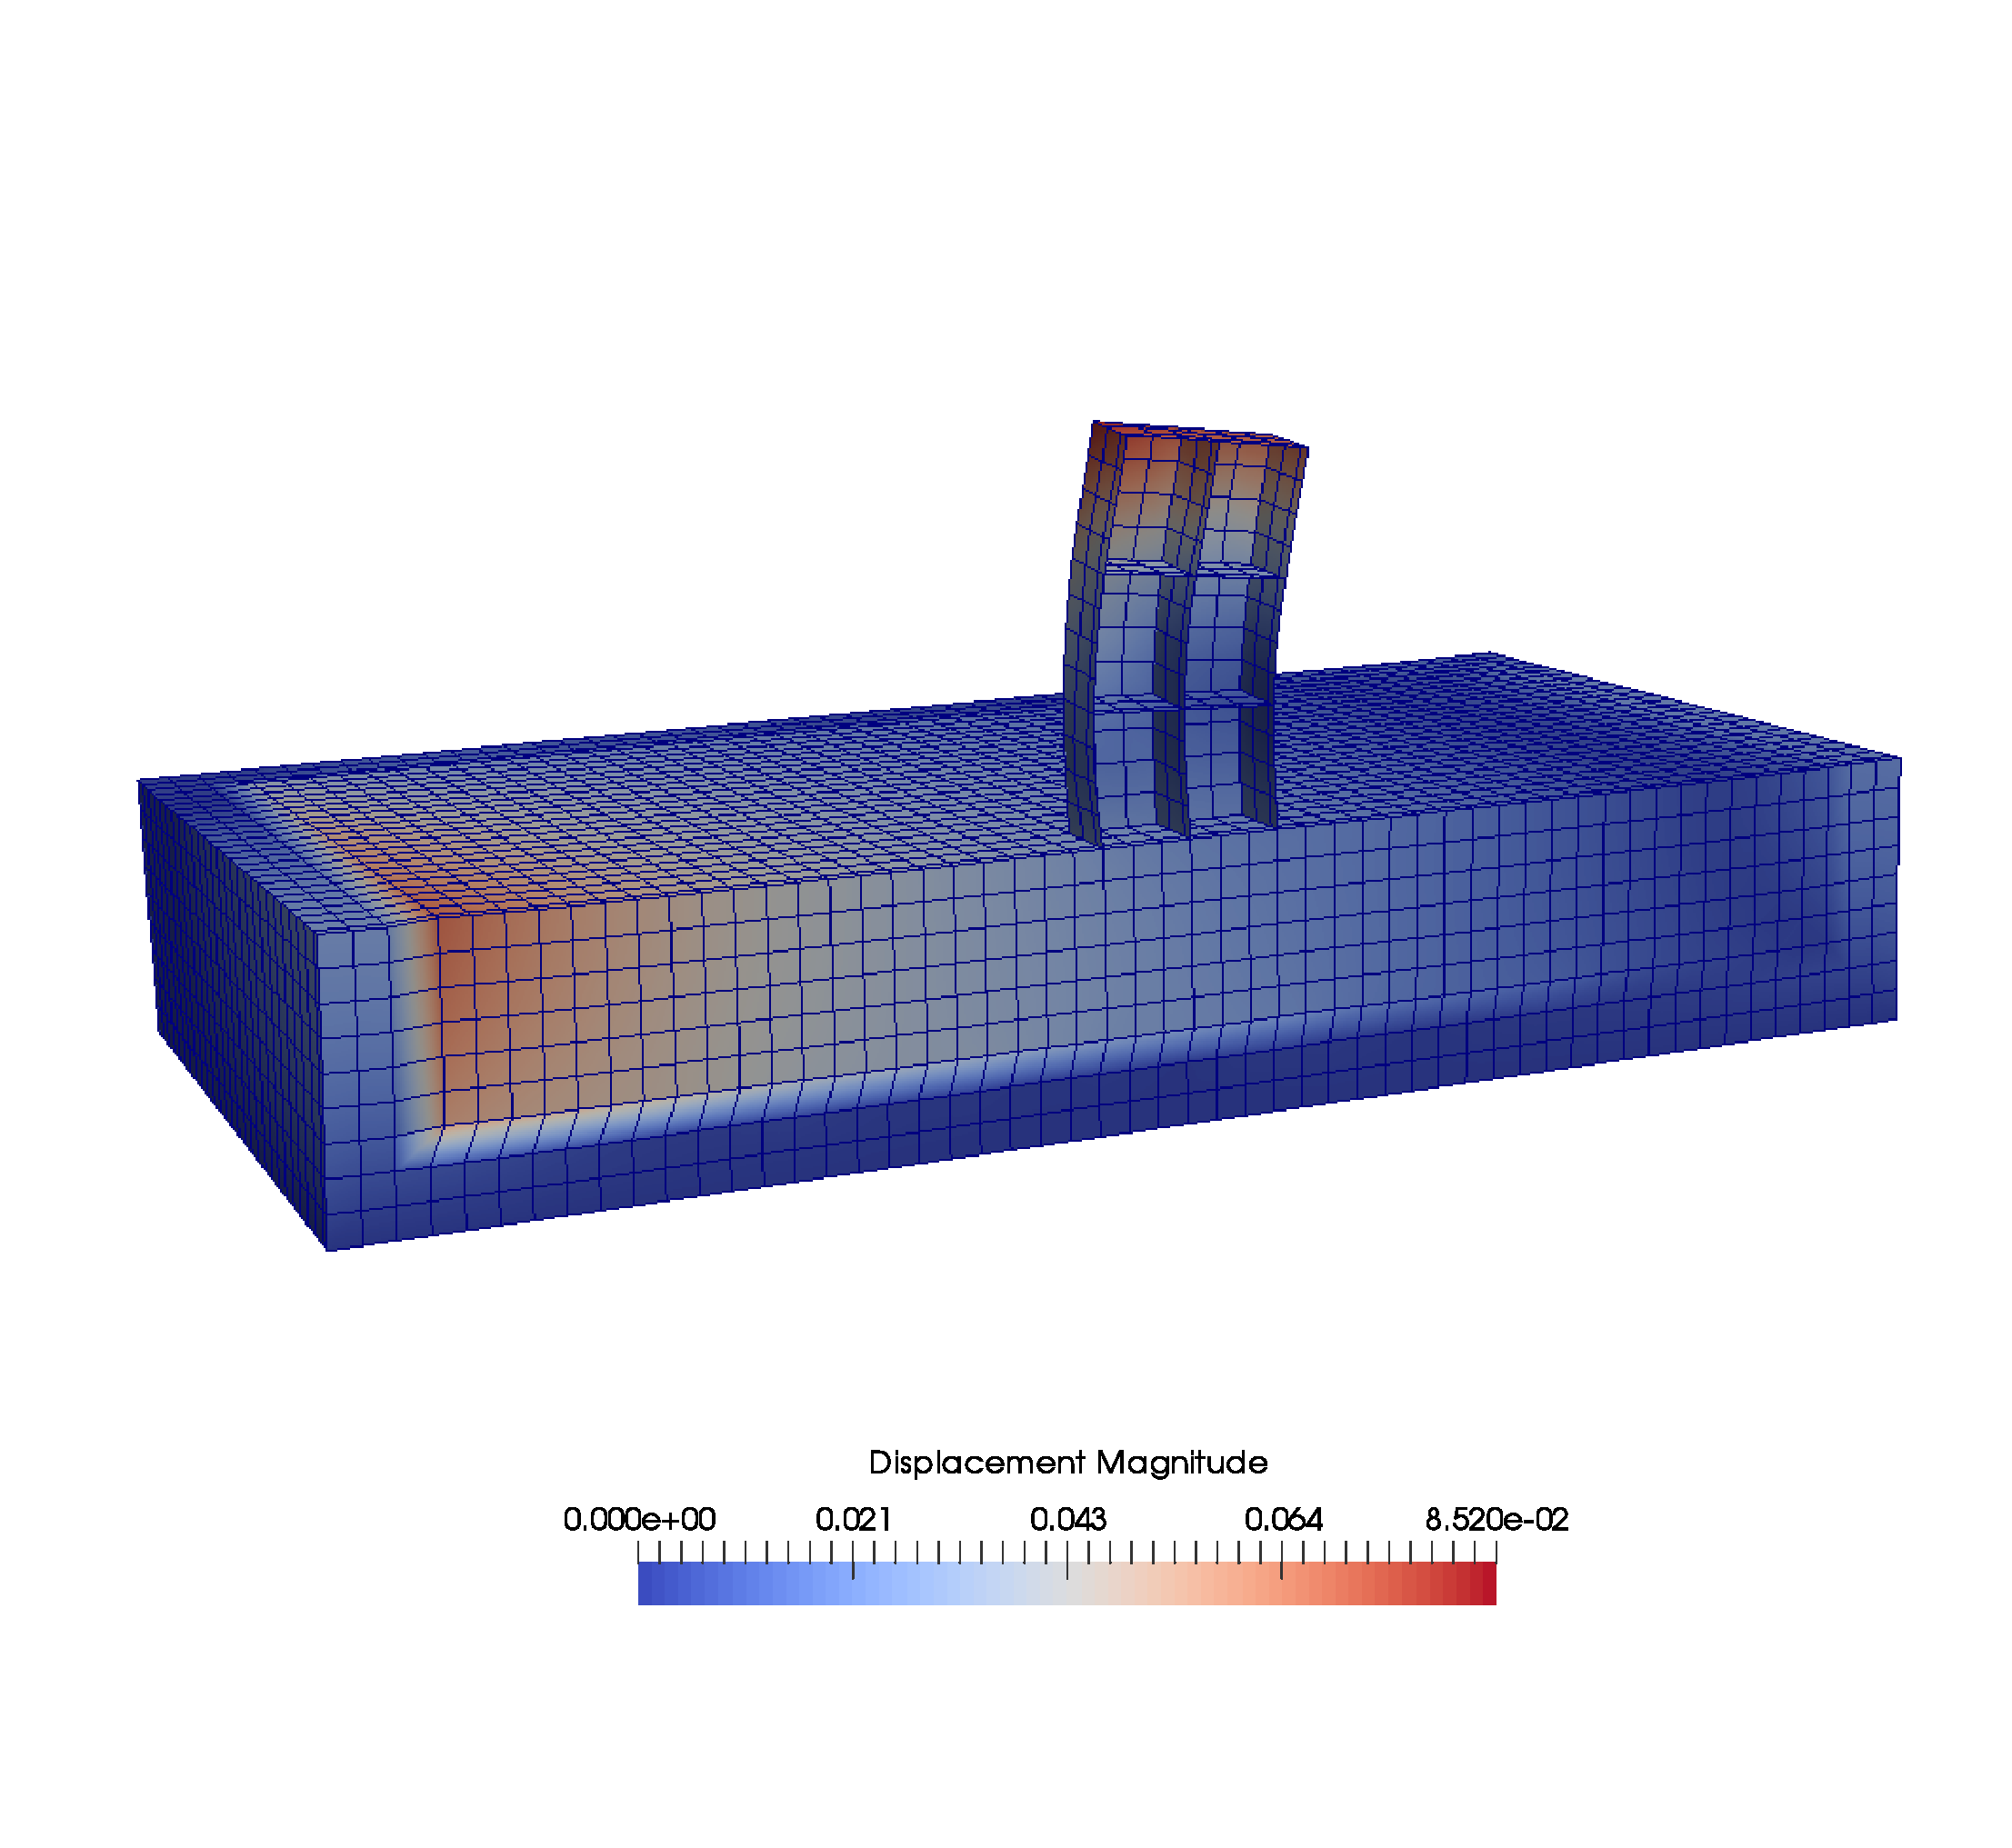
\includegraphics[width = 10cm]{./Figure-files/Day2/Apply_3D_Motions_from_SW4/Shell_Structure_Soil_Interaction_3D_DRM/3D_shell_3D_motion.pdf}
%   \caption{Simulation of 3D shell model under 3D motions}
%   \label{3D shell model under 3D seismic motion}
% \end{figure}

